\documentclass[12pt,a4paper]{article}
\usepackage[a4paper, left=3.5cm, right=2cm, top=2.5cm, bottom=3cm,footskip=.25in]{geometry}
\usepackage[utf8]{inputenc}
\usepackage[T1]{fontenc}
\usepackage{amsmath}
\usepackage{amssymb}
\usepackage{lmodern}
\usepackage{indentfirst}
\usepackage{enumerate}
\usepackage{array}
\usepackage{float}
\usepackage{ragged2e}
\usepackage{lipsum}
\usepackage{titlesec}
\usepackage[pdftex]{graphicx}
\graphicspath{{.png}{images/}}
\renewcommand{\baselinestretch}{1.8}

\usepackage{pdfpages}

\usepackage{hyperref}
\hypersetup{colorlinks=true, linkcolor=black}

\titlespacing*{\section}
{0pt}{5.5ex plus 1ex minus .2ex}{4.3ex plus .2ex}
\titlespacing*{\subsection}
{0pt}{5.5ex plus 1ex minus .2ex}{4.3ex plus .2ex}

\usepackage{soul}
\newcommand{\ol}[1]{{\setul{-1.2em}{}\ul{#1}}}
\newcommand{\textoverline}[1]{{\setul{-5em}{}$\overline{\mbox{#1}}$}}

\newtheorem{definition}{Definition}[subsection]
\newtheorem{example}{Example}[subsection]

\usepackage[round]{natbib}
\usepackage{tikz-qtree}
\usepackage{tikz}
\usetikzlibrary{arrows}
\usetikzlibrary{decorations.text}

\usepackage{pifont}
\newcommand{\xmark}{\ding{53}}

\begin{document}

\begin{titlepage}
	\centering
	\par\vspace{1cm}
	{\scshape\bf FACULTY OF MATHEMATICS, PHYSICS AND INFORMATICS \par}
	{\scshape\bf OF THE COMENIUS UNIVERSITY IN BRATISLAVA \par}
	\par\vspace{8cm}
	{\scshape\bf OPTIMIZATION OF AN ABDUCTIVE REASONER FOR DESCRIPTION LOGICS \par}
	\par\vspace{0.5cm}
	{\textsc Master thesis \par}
	\par\vspace{10.6cm}
	{\scshape\bf 2019 \hfill Katarína Fabianová \par}
\end{titlepage}

\pagebreak
\thispagestyle{empty}
\centering
\par\vspace{1cm}
{\scshape\bf FACULTY OF MATHEMATICS, PHYSICS AND INFORMATICS \par}
{\scshape\bf OF THE COMENIUS UNIVERSITY IN BRATISLAVA \par}
\par\vspace{8cm}
{\scshape\bf OPTIMIZATION OF AN ABDUCTIVE REASONER FOR DESCRIPTION LOGICS \par}
\par\vspace{0.5cm}
{\textsc Master thesis \par}
\par\vspace{2cm}
\begin{table*}[ht]
	\newcolumntype{x}[1]{>{\hspace{0pt}}p{#1}}
	\begin{tabular}{@{}x{5cm}x{10cm}@{}}
		Study program: & Applied informatics \\
		Field of study: & 2511 Applied informatics \\
		School department: & Department of Applied Informatics \\
		Adviser: & Mgr. Júlia Pukancová, PhD. \\
		Consultant: & RNDr. Martin Homola, PhD. \\
	\end{tabular}
\end{table*}
\par\vspace{3.03cm}
{\scshape\bf Bratislava 2019 \hfill Katarína Fabianová \par}

\pagebreak

\justify

%\pagebreak
%\thispagestyle{empty}
%\par\vspace*{15cm}
%{\large\bf Dedication \par}
%\par\vspace{0.8cm}
%\large Čestne prehlasujem, že prácu som vypracovala samostatne
%pod vedením školiteľa a uviedla som všetky použité
%zdroje informácií a použitú literatúru. \par
%\par\vspace{3cm}
%\large {Bratislava \hfill \textoverline{Katarína Fabianová}} \par

\pagebreak
\thispagestyle{empty}
\par\vspace*{15cm}
{\large\bf Acknowledgements \newline \par}

\pagebreak
\thispagestyle{empty}
{\large\bf Abstract \newline \par} 

\textbf{Key words:}

\pagebreak
\thispagestyle{empty}
{\large\bf Abstrakt \newline \par} 

\textbf{Kľúčové slová:}

\pagebreak
\thispagestyle{empty}
\tableofcontents
\thispagestyle{empty}

\pagebreak
\thispagestyle{empty}
\listoffigures

\pagebreak
\section*{Introduction}
\addcontentsline{toc}{section}{\protect\numberline{}Introduction}


\pagebreak
\section{Description logics}
Description logics (DLs) are a family of knowledge representation formalism. Each description logic has different expressivity. Every expressivity is expressed with a unique set of constructors. We are going to work with $\mathcal{ALC}$, $\mathcal{EL}$ and $\mathcal{EL}${+}{+} DL. Each description logic has its own syntax and semantics. In this chapter we will introduce syntax and semantics \citep{Rudolph2011} for each DL that we will be working with.

\subsection{$\mathcal{ALC}$ DL}
$\mathcal{ALC}$ DL is a DL which is more expressive than $\mathcal{EL}$ and $\mathcal{EL}{+}{+}$ DL. $\mathcal{ALC}$ is less expressive than many other DLs. $ALC$ stands for Attributive (Concept) Language with Complements. It means that not only complement of atomic concept is allowed but also a complement of complex concept is allowed.

\subsubsection{$\mathcal{ALC}$ Syntax}
$\mathcal{ALC}$ description logic consists of three mutually disjoint sets. These sets represent whole domain that is used by $\mathcal{ALC}$ DL.

\begin{definition}{\textbf{DL vocabulary}}
	\[ \textbf{Set of individuals:} N_{I} = \{a,b,c...\} \]
	\[ \textbf{Set of concepts:} N_{C} = \{A,B,C...\} \]
	\[ \textbf{Set of roles:} N_{R} = \{R_{1},R_{2},R_{3},...\} \]
\end{definition}

\begin{example}{\textbf{DL vocabulary}}
	\[ Individuals = \{ jack, john, jane \} \]
	\[ Concepts = \{ Person, Mother, Father \} \]
	\[ Roles = \{ hasChild, likes, owns \} \]
\end{example}

$\mathcal{ALC}$ DL deals with individuals and concepts. An individual is a concrete instance of a concept. Concept is a class that defines some entity. Concept can have two forms, one is concept assertion and the second one is role assertion.

Concept can be atomic or complex. Atomic concept is not constructed with any constructor. On the contrary complex concept is created from constructors and other concepts.

\begin{definition}{\textbf{Complex concept}}
	
	Concepts are recursively constructed as the smallest set of expressions of the forms:
	\[ C,D ::= A | \neg C | C \sqcap D | C \sqcup D | \exists R.C | \forall R.C \]
	where $A \in N_{C}$, $R \in N_{R}$, and C, D are concepts.
\end{definition}

\begin{example}{\textbf{Complex concept}}
\[ \neg Mother \]
\[ Mother \sqcup Father \]
\[ \exists hasChild.Person \]
\[ \forall likes.Food \]
\end{example}

Complex concept uses following constructors: $\neg$, $\sqcup$, $\sqcap$, $\exists$ and $\forall$. Constructor $\neg$ means negation, constructor $\sqcup$ means or and constructor $\sqcap$ means and. Constructors $\exists$ is existential restriction and $\forall$ is called value restriction.

There are two concepts that are always in ontology. $\top$ (top) stays for everything. Each concept belongs under $\top$ which means that each concept is on left side of subsumption if on right side is only $\top$. Second concept is $\bot$ (bottom) and it stays for nothing which means that each concept is on the right side of subsumption if there is only $\bot$ on the left side. Formally these two concepts can be written as follows:
\[ \top \equiv A \sqcup \neg A \]
\[ \bot \equiv A \sqcap \neg A \]

$\mathcal{ALC}$ description logic uses axioms in order to model some situation. There are two types of axioms, first is TBox and the second one is ABox. In TBox is used symbol $\sqsubseteq$. Let's explain this symbol on an example $Mother \sqsubseteq Parent$. $Mother$ is always a $Parent$ but $Parent$ does not always have to be a $Mother$. 

\begin{definition}{\textbf{TBox}}
	
	A TBox $\mathcal{T}$ is a finite set of GCI axioms $\phi$ of the form:
	\[ \phi ::= C \sqsubseteq D \]	
	where C, D are any concepts.
\end{definition}

\begin{example}{\textbf{TBox}}
	\[ 
	\mathcal{T} = \left\{
	\begin{tabular}{c c}
	$Professor \sqcup Scientist \sqsubseteq Academician$ \\
	$AssocProfessor \sqsubseteq Professor$ \\
	\end{tabular}
	\right \}
	\]
\end{example}

\begin{definition}{\textbf{ABox}}
	
    An ABox $\mathcal{A}$ is a finite set of assertion axioms $\phi$ of the form:
	\[ \phi ::= a:C | a,b:R \]
	where $a,b \in N_{I}$, $R \in N_{R}$ and C is any concept.
\end{definition}

\begin{example}{\textbf{ABox}}
	\[ 
	\mathcal{A} = \left\{
	\begin{tabular}{c c}
	$jack : Academician$ \\
	$jane : Scientist$ \\
	$john : Professor$ \\
	\end{tabular}
	\right \}
	\]
\end{example}

To have a better understanding of $\mathcal{ALC}$ DL we can translate sentences into $\mathcal{ALC}$ description logic.

\[ \text{Everybody who is sick, is not happy.} \]
\[ Sick \sqsubseteq \neg Happy \]

\[ \text{Cat and dogs are animals.} \]
\[ Cat \sqcup Dog \sqsubseteq Animal \]

\[ \text{Every person owns a house.} \]
\[ Person \sqsubseteq \exists owns.House \]

\subsubsection{$\mathcal{ALC}$ Semantics}
Ontology \citep{staabHandbookOntology} describes relationships between entities in a specific area. Difference between area and ontology is that ontology describes relationships between entities in a formal language.

Every ontology has its own knowledge base. Knowledge base is a set of TBox axioms and ABox axioms. Ontology is described by knowledge base. TBox represents axioms that model ontology. Each axiom explains the relationship between entities in this axiom. ABox on the other side does not model ontology but creates a database of facts. It contains set of assertion axioms that can be called facts. Fact is a direct assertion of an individual to a concept.

\begin{definition}{\textbf{Knowledge base}}
	
Knowledge base ($\mathcal{KB}$) is an ordered pair of \textit{TBox} $\mathcal{T}$ and \textit{ABox} $\mathcal{A}$.
\end{definition}

\begin{example}{\textbf{Knowledge base}}
	\[ 
	\mathcal{KB} = \left\{
	\begin{tabular}{c c}
	$Professor \sqcup Scientist \sqsubseteq Academician$ \\
	$AssocProfessor \sqsubseteq Professor$ \\
	$jack : Academician$ \\
	$jane : Scientist$ \\
	$john : Professor$ \\	
	\end{tabular}
	\right \}
	\]
\end{example}

An interpretation is a pair of domain and interpretation function. Domain is a set of values that represents concepts in the interpretation. Result of interpretation function is different for individuals, concepts and roles. If we use interpretation function on individual the result is an element from domain. If we use it on concepts the result is a set of elements from domain. If we use it on roles the result is a pair of elements from domain.

\begin{definition}{\textbf{Interpretation}}

	An interpretation of a given knowledge base $\mathcal{KB} = (\mathcal{T}, \mathcal{A})$ is a pair $\mathcal{I} = (\Delta^{\mathcal{I}}, \cdot ^{\mathcal{I}})$ which contains a domain $\Delta^{\mathcal{I}}$ and an interpretation function $\cdot ^{\mathcal{I}}$.	
	Domain can not be empty. So it must be true that $\Delta^{\mathcal{I}} \not = \emptyset$.
		
	The interpretation function is following:
	\[ a^{\mathcal{I}} \in \Delta^{\mathcal{I}} \text{ } \forall a \in N_{I} \]
	\[ A^{\mathcal{I}} \subseteq \Delta^{\mathcal{I}} \text{ } \forall A \in N_{C} \]
	\[ R^{\mathcal{I}} \subseteq \Delta^{\mathcal{I}} \times \Delta^{\mathcal{I}} \text{ } \forall R \in N_{R} \]
	The interpretation of complex concepts is recursively defined:
	\[ \neg C^{\mathcal{I}} = \Delta^{\mathcal{I}} \backslash C^{\mathcal{I}} \]
	\[ C \sqcap D^{\mathcal{I}} = C^{\mathcal{I}} \cap D^{\mathcal{I}} \]
	\[ C \sqcup D^{\mathcal{I}} = C^{\mathcal{I}} \cup D^{\mathcal{I}} \]
	\[ \exists R.C^{\mathcal{I}} = \{ x \in \Delta^{\mathcal{I}} | \exists y \in \Delta^{\mathcal{I}} : \langle x,y \rangle \in R^{\mathcal{I}} \land y \in C^{\mathcal{I}} \} \]
	\[ \forall R.C^{\mathcal{I}} = \{ x \in \Delta^{\mathcal{I}} | \forall y \in \Delta^{\mathcal{I}} : \langle x,y \rangle \in R^{\mathcal{I}} \rightarrow y \in C^{\mathcal{I}} \} \]
\end{definition}

\begin{example}{\textbf{Interpretation}}
	\[ 
	\mathcal{KB} = \left\{
	\begin{tabular}{c c}
	$Professor \sqcup Scientist \sqsubseteq Academician$ \\
	$AssocProfessor \sqsubseteq Professor$ \\
	$jack : Academician$ \\
	\end{tabular}
	\right \}
	\]
	
	\[ \mathcal{I} = (\Delta ^{\mathcal{I}}, \cdot^{\mathcal{I}}) \]
	\[ \Delta ^{\mathcal{I}} = \{ P,S,A,AP \} \]
	\[ Professor^{\mathcal{I}} = \{P\} \]
	\[ Scientist^{\mathcal{I}} = \{S\} \]
	\[ Academician^{\mathcal{I}} = \{A\} \]
	\[ AssocProfessor^{\mathcal{I}} = \{AP\} \]
	\[ jack^{\mathcal{I}} = A \]
	
\end{example}

The interpretation satisfies an axiom according to its type. We know three types of axioms. First is an axiom from TBox, second is assertion axiom to a concept and the third one is an assertion to a role.

\begin{definition}{\textbf{Satisfaction $\models$}}

	Given an axiom $\phi$, an interpretation $\mathcal{I} = (\Delta^{\mathcal{I}}, \cdot ^{\mathcal{I}})$ satisfies $\phi (\mathcal{I} \models \phi)$ depending on its type:
	\[ C \sqsubseteq D: \mathcal{I} \models C \sqsubseteq D \text{ iff } C^{\mathcal{I}} \subseteq D^{\mathcal{I}} \]
	\[ a:C: \mathcal{I} \models a:C \text{ iff } a^{\mathcal{I}} \in C^{\mathcal{I}} \]
	\[ a,b:R: \mathcal{I} \models a,b:R \text{ iff } \langle a^{\mathcal{I}}, \in b^{\mathcal{I}} \rangle \in R^{\mathcal{I}} \]	
\end{definition}

Finding a model is crucial for consistency checking. If we find at least one model knowledge base $\mathcal{KB}$ is consistent. We can have more models for one knowledge base. In Example 1.1.7 there are two showed models but there can be more models. 

\begin{definition}{\textbf{Model}}
	
	An interpretation $\mathcal{I} = \langle \Delta^{\mathcal{I}}, \cdot ^{\mathcal{I}}  \rangle$ is a model of a DL knowledge base $\mathcal{KB} = (\mathcal{T}, \mathcal{A})$ iff $\mathcal{I}$ satisfies every axiom in TBox $\mathcal{T}$ and ABox $\mathcal{A}$.
\end{definition}

\begin{example}{\textbf{Model}}
	\[ 
	\mathcal{KB} = \left\{
	\begin{tabular}{c c}
	$Professor \sqcup Scientist \sqsubseteq Academician$ \\
	$AssocProfessor \sqsubseteq Professor$ \\
	$jack : Academician$ \\
	\end{tabular}
	\right \}
	\]

	\[ \mathcal{M}_{1} = \{  \Delta^{\mathcal{I}} = \{ P,S,A,AP \}, \]	
	\[ Professor^{\mathcal{I}} = \{P\}, Scientist^{\mathcal{I}} = \{S\}, Academician^{\mathcal{I}} = \{A\}, AssocProfessor^{\mathcal{I}} = \{AP\} \]
	\[ jack^{\mathcal{I}} = A \} \]	

	\[ \mathcal{M}_{2} = \{  \Delta^{\mathcal{I}} = \{ A \}, \]	
	\[ Professor^{\mathcal{I}} = \{A\}, Scientist^{\mathcal{I}} = \{A\}, Academician^{\mathcal{I}} = \{A\}, AssocProfessor^{\mathcal{I}} = \{A\} \]
	\[ jack^{\mathcal{I}} = A \} \]		
\end{example}

\begin{definition}{\textbf{Consistency}}
	
	A knowledge base $\mathcal{KB}$ is consistent iff $\mathcal{KB}$ has at least one model $\mathcal{M}$.
\end{definition}

We are familiar with four decision problems, satisfiability, subsumption $(\sqsubseteq)$, equivalence ($\equiv$) and disjointness. Satisfiability means that concept is satisfiable in regard to $\mathcal{KB}$ if we can find such a model of knowledge base for which holds that interpretation of that concept is not empty. Subsumption between two concepts means that it must hold that interpretation of left-sided concept is a proper subset of interpretation of right-sided concept in each possible model of knowledge base. Equivalence is similar to subsumption but the difference is that the interpretations of both concepts must be equal in each possible model of knowledge base. Disjointness means that intersection of the interpretations of both concepts must be empty set in each possible model of knowledge base.

\begin{definition}{\textbf{Decision problems}}

	Given a DL $\mathcal{KB} = (\mathcal{T}, \mathcal{A})$, and two concepts C,D, we say that:

	\begin{itemize}
		\item $C \text{ is satisfiable w.r.t. } \mathcal{KB} \text{ iff there is such a model } \mathcal{I} \text{ of } \mathcal{KB} \text{ for which holds that } \newline C^{\mathcal{I}} \neq \emptyset;$

		\item $C \text{ is subsumed by D w.r.t. } \mathcal{KB} \text{ (denoted } \mathcal{KB} \models C \sqsubseteq D) \text{ iff } C^{\mathcal{I}} \subseteq D^{\mathcal{I}} \text{ in every} \newline \text{model } \mathcal{I} \text{ of } \mathcal{KB};$

		\item $\text{C and D are equivalent w.r.t. } \mathcal{KB} \text{ (denoted } \mathcal{KB} \models C \equiv D) \text{ iff } C^{\mathcal{I}} = D^{\mathcal{I}} \text{ in every} \newline \text{model } \mathcal{I} \text{ off } \mathcal{KB};$
		
		\item $\text{C and D are disjoint w.r.t. } \mathcal{KB} \text{ iff } C^{\mathcal{I}} \cap D^{\mathcal{I}} = \emptyset \text{ in every model } \mathcal{I} \text{ off } \mathcal{KB}.$		
	\end{itemize}
\end{definition}

If $\mathcal{KB} = \emptyset$ then we say that decision problems (satisfiability, subsumption, equivalence and disjointness) of concepts are defined in general by definition and we use notation such as we omit $\mathcal{KB} \models$ from the notation.

\subsection{DL Tableau algorithm}
DL Tableau algorithm proves satisfiability if input is concept C and TBox $\mathcal{T}$. But if input is knowledge base $\mathcal{KB}$ then this algorithm is modified to check consistency of given knowledge base. In both versions of this algorithm holds that each concept must be in NNF (negation normal form). Negation normal form is such a form that each negation is pushed in front of atomic concept inside a complex concept. DL Tableau algorithm creates a CTree (Completion tree). At first it initializes with input concept if it proves concept satisfiability otherwise it creates a named node and continue with input concept and then applies tableau rules for given DL. If the algorithm finds a clash in some node, created CTree is not clash-free and the result is that C is unsatisfiable w.r.t. $\mathcal{T}$. If the algorithm applies each rule until any rule can be applied and it finds no clash then result is that concept C is satisfiable w.r.t. $\mathcal{T}$. Following definitions \citep{baaderHandbook} are describing rules and terms that are used by this algorithm.

\begin{definition}{\textbf{NNF}}

	A concept C is in NNF (negation normal form) iff the complement constructor $\neg$ 
	only occurs in front of atomic concept symbols inside C.
\end{definition}

\begin{example}{\textbf{NNF}}
	\[ \neg (C \sqcap D) \equiv \neg C \sqcup \neg D \]
	\[ \neg (C \sqcup D) \equiv \neg C \sqcap \neg D \]
	\[ \neg \exists R.C \equiv \forall R. \neg C \]
	\[ \neg \forall R.C \equiv \exists R. \neg C \]
\end{example}

\begin{definition}{\textbf{Completion tree}}

	A completion tree (CTree) is a triple T = (V, E, $\mathcal{L}$) where (V, E)
	is a tree and $\mathcal{L}$ is a labeling function which means that:
	$\mathcal{L}(x)$ is a set of concepts $\forall x \in V$ and
	$\mathcal{L}(\langle x, y \rangle )$ is a set of roles $\forall \langle x, y \rangle \in E$.	
\end{definition}

\begin{definition}{\textbf{Successor, R-successor}}

	Given a CTree T = (V,E, $\mathcal{L}$) and $x,y \in V$ we say that: 
	\begin{itemize}
		\item y is a successor of x iff $\langle x,y \rangle \in E$
		\item y is an R-successor of x iff $\langle x,y \rangle \in E$ and $R \in \mathcal{L}(\langle x,y \rangle)$.
	\end{itemize}
\end{definition}

\begin{definition}{\textbf{Clash}}

	There is a clash in a CTree T = $(V,E, \mathcal{L})$ if and only iff for some $x \in V$ and for some concept C both $C \in \mathcal{L}(x)$ and $\neg C \in \mathcal{L}(x)$.
\end{definition}

\begin{example}{\textbf{Clash}}
	\[ \mathcal{L}(s_{0}) = \{ C, D, \neg D \} \]
\end{example}

\begin{definition}{\textbf{Clash-free CTree}}

A CTree T = $(V,E, \mathcal{L})$ is clash-free iff none of the nodes in V contains a clash.
\end{definition}

\begin{definition}{\textbf{Blocking}}
	
	Given a CTree $T = (V, E, \mathcal{L})$ a node $x \in V$ is blocked if it has an ancestor $y$ such that: either $\mathcal{L}(x) \subseteq \mathcal{L}(y)$ or $y$ is blocked.
\end{definition}

DL Tableau algorithm proves concept satisfiability in regard of TBox. Input for DL Tableau algorithm is concept C and TBox $\mathcal{T}$. Output is a boolean value which is true if concept C is satisfiable w.r.t. $\mathcal{T}$, false otherwise.

\begin{definition}{\textbf{Algorithm - Concept satisfiability}}	
	
	\noindent \textbf{Input:} concept C and $\mathcal{T}$ in NNF \newline
	\textbf{Output:} answers if concept C is satisfiable w.r.t. $\mathcal{T}$ or not \newline
	\textbf{Steps:}
	\begin{enumerate}
		\item Initialize a new CTree T := $(\{s_{0}\}, \emptyset, \{s_{0} \rightarrow \{C\}\})$;
		\item Apply tableau rules for TBoxes while at least one rule is applicable;
		\item Answer "C is satisfiable w.r.t. $\mathcal{T}$" if T is clash-free. Otherwise answer "C is unsatisfiable w.r.t. $\mathcal{T}$".
	\end{enumerate}
\end{definition}	

\begin{definition}{\textbf{$\mathcal{ALC}$ tableau rules for TBoxes}}
	\begin{itemize}
		\item $\sqcap-rule:$ if $C_{1} \sqcap C_{2} \in \mathcal{L}(x)$ and $x \in V$ and $\{ C_{1}, C_{2} \} \not \subseteq \mathcal{L}(x)$ and x is not blocked then $\mathcal{L}(x) = \mathcal{L}(x) \cup \{ C_{1}, C_{2} \}$
		
		\item $\sqcup-rule:$ if $C_{1} \sqcup C_{2} \in \mathcal{L}(x)$ and $x \in V$ and $ \{ C_{1}, C_{2} \} \cap \mathcal{L}(x) = \emptyset$ and x is not blocked then either $\mathcal{L}(x) = \mathcal{L}(x) \cup \{ C_{1} \}$ or $\mathcal{L}(x) = \mathcal{L}(x) \cup \{ C_{2} \}$
		
		\item $\forall-rule:$ if $\forall R.C \in \mathcal{L}(x)$ and $x,y \in V$ and y is R-successor of x and $C \not \in \mathcal{L}(y)$ and x is not blocked then $\mathcal{L}(y) = \mathcal{L}(y) \cup \{ C \}$
		
		\item $\exists-rule:$ if $\exists R.C \in \mathcal{L}(x)$ and $x \in V$ with no R-successor y and $C \in \mathcal{L}(y)$ and x is not blocked then $\mathcal{V} = \mathcal{V} \cup \{ z \}, \mathcal{L}(z) = \{ C\}$ and $\mathcal{L}( \langle x, z \rangle ) = \{ R \}$
		
		\item $\mathcal{T}-rule:$ if $C_{1} \sqsubseteq C_{2} \in \mathcal{T}$ and $x \in V$ and nnf$(\neg C_{1} \sqcup C_{2}) \not \in \mathcal{L}(x)$ and x is not blocked then $\mathcal{L}(x) = \mathcal{L}(x) \cup \{ nnf(\neg C_{1} \sqcup C_{2}) \}$
	\end{itemize}
\end{definition}	

Knowledge base is a pair of a TBox and an Abox and yet only a TBox was mentioned in connection with DL Tableau algorithm. If we also have a given ABox the algorithm must be modified. The algorithm no longer checks concept satisfiability w.r.t. $\mathcal{T}$ but checks consistency of given $\mathcal{KB}$. For result holds the same condition as in proving concept satisfiability. If there is a found clash knowledge base is not consistent otherwise knowledge base is consistent. Difference between the first version of this algorithm is that here are used named nodes. Name of the node is an instance of a concept that comes from ABox. 

\begin{definition}{\textbf{Algorithm - Consistency checking}}

\noindent \textbf{Input:} $\mathcal{KB} = (\mathcal{T}, \mathcal{A})$ in NNF \newline
\textbf{Output:} answers if $\mathcal{KB}$ is consistent or not \newline
\textbf{Steps:}
\begin{enumerate}
	\item Initialize a CTree as follows:
		\begin{itemize}
			\item $V := \{ a \text{ } | \text{ constant a occurs in } \mathcal{A} \}$;
			\item $E := \{ \langle a,b \rangle \text{ } | \text{ } a,b : R \in \mathcal{A} \text{ for some role R} \}$;
			\item $\mathcal{L}(a) := \{ nnf(E) \text{ } | \text{ } a:E \in \mathcal{A}\} \text{ for all } a \in V$; \newline
			$\mathcal{L}(\langle a,b \rangle) := \{ R \text{ } | \text{ } a,b:R \in \mathcal{A}\} \text{ for all } \langle a,b \rangle \in E$;
		\end{itemize}
	\item Apply tableau rules for TBoxes while at least one rule is applicable;
	\item Answer "$\mathcal{KB}$ is consistent" if T is clash-free. Otherwise answer "$\mathcal{KB}$ is inconsistent".
\end{enumerate}

\end{definition}

Let's introduce an example where we know a knowledge base $\mathcal{KB}$. DL Tableau algorithm checks if knowledge base is consistent or not.

\begin{example}{(\textbf{DL Tableau algorithm})}
	\[ 
	\mathcal{KB} = \left\{
	\begin{tabular}{c c}
	$Student \sqsubseteq \exists attends.Logic$ \\
	$Logic \sqsubseteq Course$ \\
	$jack : Student$ \\
	\end{tabular}
	\right \}
	\] \\
\end{example}

\begin{center}
	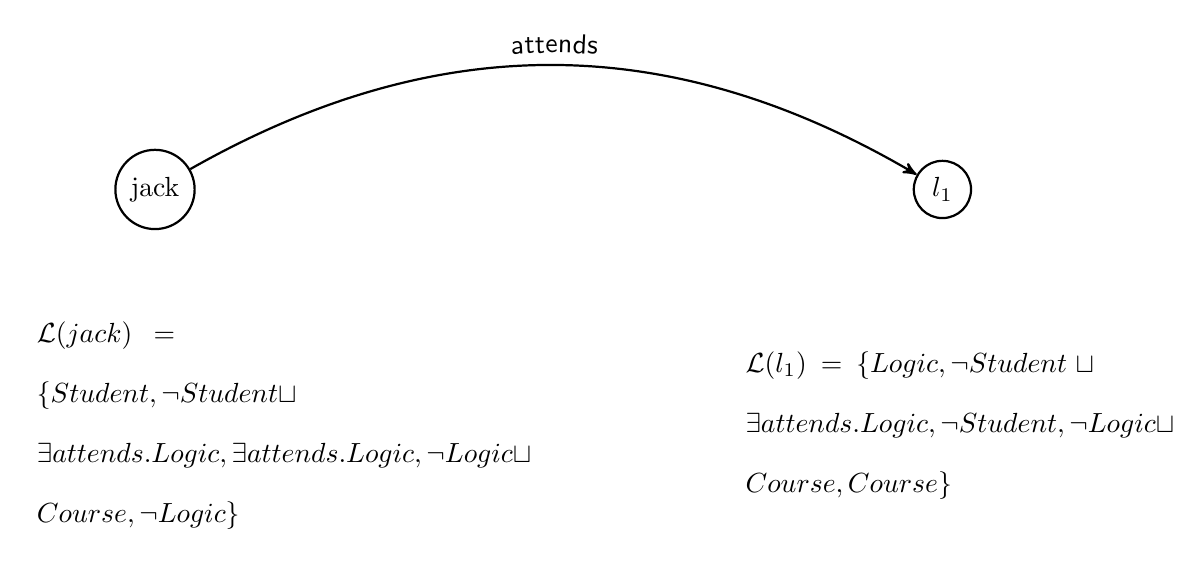
\begin{tikzpicture}[->,>=stealth',auto,node distance=10cm,
	thick,main node/.style={circle, draw}]
	
	\node[main node] (1) {jack};
	\node[main node] (2) [right of=1] {$l_{1}$};
	
	\def\myshift#1{\raisebox{1ex}}
	
	\draw [thick, ->, postaction={decorate, decoration={text along path, text align=center, text={|\sffamily\myshift|attends}}}] (1) to [bend left=30] (2);
	
	\node[text width=3cm] at (0,-3) 
	{$\mathcal{L}(jack) = \{ Student, \neg Student \sqcup \exists attends.Logic, \exists attends.Logic, \neg Logic \sqcup Course, \neg Logic \}$};		

	\node[text width=5cm] at (10,-3) 
	{$\mathcal{L}(l_{1}) = \{ Logic, \neg Student \sqcup \exists attends.Logic, \neg Student, \neg Logic \sqcup Course, Course \}$};			
	\end{tikzpicture}
\end{center}

The algorithm starts with ABox assertion axioms. It selects axiom $jack : Student$.
At first it creates a node $jack$ with its label $\mathcal{L}(jack)$. From the assertion axiom $jack : Student$ algorithm knows that jack is a Student and add to the label $\mathcal{L}(jack)$ concept $Student$. Then the algorithm is choosing another axiom from knowledge base. There are no more assertion axioms, so it starts with axioms from TBox. It will take $Student \sqsubseteq \exists attends.Logic$. It must convert it into negation normal form which will be $\neg Student \sqcup \exists attends.Logic$. The algorithm is applying $\sqcup-rule$. According this rule it must choose $\exists attends.Logic$, otherwise there would be a clash. Now it has to apply $\exists - rule$ so a new node $l_{1}$ will be created with its label $\mathcal{L}(l_{1})$. Into this label $\mathcal{L}(l_{1})$ will be added concept $Logic$. Let's go back to $jack$ node. The algorithm has to finish adding all axioms of TBox form. It will add the second axiom from knowledge base in negation normal form as $\neg Logic \sqcup Course$. Now it does not matter which one algorithm chooses if $Course$ or $\neg Logic$ because any of these two does not cause a clash. Now the algorithm goes back to $l_{1}$ node and continues to add axioms from knowledge base similarly as in node $jack$. It starts with axiom $\neg Student \sqcup \exists attends.Logic$, it will choose the first one $\neg Student$. Then continues with axiom $\neg Logic \sqcup Course$. It can not choose $\neg Logic$ because there would be immediately a clash. So it chooses $Course$.

The created tree contains two nodes ($jack$ and $l_{1}$) and one edge between them. The edge represents that $jack$ attends some Logic $l_{1}$. There is not any instance of a concept $Logic$ so node $l_{1}$ does not represent a concrete instance of concept $Logic$ but represents some instance. There is no clash in both nodes so the answer of DL Tableau algorithm is that given knowledge base $\mathcal{KB}$ is consistent.

\section{Abduction}
Generally in logic we are familiar with three ways of thinking. Deduction, induction and abduction. The most known and natural for humans is probably deduction. All three ways are dealing with following parts: theory, data and effect. In description logic we can translate theory as knowledge base, data as explanations and  effect as observation.

Deduction knows knowledge base and explanations, observation is missing and the goal is to deduce the missing observation. Induction knows observation and explanation but does not know knowledge base. Abduction knows knowledge base and observation but explanation is a subject of searching. All definitions are from article by \citep{pukancovaAboxAbduction}.

\subsection{ABox abduction}
In description logic abduction is used when we are not familiar with explanation $\mathcal{E}$ but we know knowledge base $\mathcal{KB}$ and observation $\mathcal{O}$. It is important to know that we are looking for minimal explanations. Minimal explanation is such an explanation that it does not exist any other explanation that would be a subset of this minimal explanation.

\begin{definition}{\textbf{(Abduction)}} 

	Given knowledge base $\mathcal{KB}$ and observation $\mathcal{O}$, an abductive explanation is such explanation $\mathcal{E}$ that satisfies $\mathcal{KB} \cup \mathcal{E} \models \mathcal{O}$.
\end{definition}

\begin{definition}{\textbf{(Correct explanation)}}
	\[ \mathcal{E} \text{ is consistent if } \mathcal{E} \cup \mathcal{KB} \not \models \mathcal{\bot}; \] 
	\[ \mathcal{E} \text{ is relevant if } \mathcal{E} \not \models \mathcal{O}; \]
	\[ \mathcal{E} \text{ is explanatory if } \mathcal{KB} \not \models \mathcal{O} \]
\end{definition}

\begin{definition}{\textbf{(Minimal explanation)}}
	
	Minimal explanation is such an explanation that it does not exist any other explanation that would be a subset of this explanation.
\end{definition}

For better understanding of what ABox abduction is let's introduce a few examples. First example is easy, searched explanation is obvious but it will demonstrate the problem. Second example is not so obvious that's why we have to use an algorithm to compute the solution. For computing the solution we use \textbf{Minimal Hitting Set algorithm}.

\begin{example}{(\textbf{ABox Abduction - Emotion})}
	\[ 
	\mathcal{KB} = \left\{
	\begin{tabular}{c c}
	$Sick \sqsubseteq \neg Happy$
	\end{tabular}
	\right \}
	\]
	
	\[ 
	\mathcal{O} = \left\{
	\begin{tabular}{c c}
	$mary : \neg Happy$
	\end{tabular}
	\right \}
	\]								
\end{example}

In this example we are searching for explanations. In this easy assignment is obvious that what we are looking for is that Mary must be sick. If Mary is not happy she must be sick. Formally written solution to this abduction problem is following:
\[ 
\mathcal{E} = \left\{
\begin{tabular}{c c}
$mary : Sick$
\end{tabular}
\right \}
\]

\begin{example}{(\textbf{ABox Abduction - Academy})}
	\[ 
	\mathcal{KB} = \left\{
	\begin{tabular}{c c}
		$Professor \sqcup Scientist \sqsubseteq Academician$ \\
		$AssocProfessor \sqsubseteq Professor$ \\
	\end{tabular}
	\right \}
	\]
	
	\[ 
	\mathcal{O} = \left\{
	\begin{tabular}{c c}
		$jack : Academician$
	\end{tabular}
	\right \}
	\]								
	
\end{example}

If $jack$ is an Academician he must be Professor or Scientist. If he is an Professor he must be also an AssocProfessor. This is an oversimplified explanation how we can retrieve correct explanations. For better introduction into this algorithm we will explain it step by step. We know the observation so we know that jack is an Academician, that is a fact. In our first axiom in TBox is written that if somebody is an Academician he is also a Professor or Scientist. He can be both but at least one of them but that we are not able to determine. That is why are both correct explanations. The second axiom claims that if somebody is a Professor he must be also an AssocProfessor. In this part we are not explaining the whole algorithm yet because it will be explained in our next chapter Minimal Hitting Set algorithm but we need to have at least an idea of how does it work. So as we already know the correct explanations are following:

\[ 
\mathcal{E} = \left\{
\begin{tabular}{c c}
	$jack : Professor$ \\
	$jack : Scientist$ \\
	$jack : AssocProfessor$ \\
\end{tabular}
\right \}
\]

\subsection{Minimal Hitting Set algorithm}
In this part we will find out about algorithm: Minimal hitting set. This algorithm is invented by Raymond \cite{reiterHS}. At first we will declare terms that we will be using.

\begin{definition}[Hitting set]
	Hitting set for a collection of sets $C$ is a set $H \subseteq U_{S \in C}$ such that $H \cap S$ is not empty set for each $S \in C$.
\end{definition}

\begin{definition}[HS-tree]
	Let $C$ be a collection of sets. An HS-tree $T$ for $C$ is a smallest edge-labeled and node-labeled tree with following properties:
	
	\begin{itemize}
		\item The root is labeled by $\checkmark$ if $C$ is empty. Otherwise the root is labeled by an arbitrary set of $C$.
		
		\item For each node $n$ of $T$, let $H(n)$ be the set of edge labels on the path in $T$ from the root to node $n$. The label for $n$ is any set $\sigma \in C$ such that $sigma \cap H(n) = \emptyset$, if such a set $\sigma$ exists. Otherwise, the label for $n$ is $\checkmark$. If $n$ is labeled by the set $\sigma$, then for each $o \in \sigma$, $n$ has a successor $n_{0}$ joined to $n$ by an edge of labeled by $o$.
	\end{itemize}
	
\end{definition}

\begin{definition}[Generate pruned HS-tree]{\indent}
	\begin{itemize}
		\item Generate the pruned HS-tree breadth-first, generating all nodes at any fixed level in the tree before descending to generate the nodes at the next level.
		
		\item Reusing node labels: If node $n$ has already been labeled by a set $S \in C$ and if $n'$ is a new node such that $H(n') \cap S = \emptyset$, then label $n'$ by $S$.
		
		\item Tree prunning:
		
		\begin{itemize}
			\item If node $n$ is labeled by $\checkmark$ and node $n'$ is such that $H(n) \subseteq H(n')$, then close the node $n'$. A label is not computed for $n'$ nor are any successor nodes generated.
			
			\item If node $n$ has been generated and node $n'$ is such that $H(n') = H(n)$, then close node $n'$.
			
			\item If nodes $n$ and $n'$ have been labeled by sets $S$ and $S'$ of $C$, respectively and if $S'$ is a proper subset of $S$, then for each $\alpha \in S - S'$ mark as redundant the edge from node $n$ labeled by $\alpha$. A redundant edge, together with the subtree beneath it, may be removed from the HS-tree while preserving the property that the resulting pruned HS-tree will yield all minimal hitting sets for $C$.
			
		\end{itemize}	
		
	\end{itemize}
	
\end{definition}

Reiter's algorithm is used to compute a minimal hitting set. Input is a set of sets. The goal of Reiter's algorithm is to compute minimal hitting set from this input. It means that the result hitting set will have intersection with each set from input.

Let's show an example with $F$ as input set and $HS$ as result.

\begin{example}{\textbf{(Minimal Hitting Set)}}
	\[  F = \{ \{a,b\}, \{b,c\}, \{a,c\}, \{b,d\}, \{b\} \} \]
	\[ HS = \{ \{a,b\}, \{b,c\} \} \]
\end{example}

As we can observe in this example the first result set has intersection with each set of $F$ and the second result set also has intersection with each set of $F$. So we can determine that these result sets are definitely minimal hitting sets. They are both minimal because there is no other set that is smaller and at the same time has intersection with each set of $F$.

For better and easier understanding of this algorithm we can visualize it and explain.

\begin{figure}[H]
	\centering
	\begin{tikzpicture}[level distance=2.5cm,sibling distance=2cm,
	draw, edge from parent path={(\tikzparentnode) -- (\tikzchildnode)}]
	\Tree
	[.\{a,b\}
		\edge node[auto=right] {a};
		[.\{b,c\} 
			\edge node[midway,left] {b};
			[.{\checkmark} ]
			\edge node[midway,right] {c};
			[.\{b,d\} 
				\edge node[midway,left] {b};
				[.{\xmark} ]
				\edge node[midway,right] {d};
				[.\{b\} 
					\edge node[midway,right] {b};
					[.{\xmark} ]
				]
			]			
		]
		\edge node[auto=left] {b};
		[.\{a,c\} 
			\edge node[midway,left] {a};
			[.{\xmark} ]
			\edge node[midway,right] {c};
			[.{\checkmark} ]
		]	
	]
	\end{tikzpicture}

	\caption{Minimal Hitting Set}
	\label{fig:MinimalHS}	
\end{figure}

Aim is to create a tree where nodes can have three types of value. Node can be set from $F$, check or cross. Each edge is labeled by one element of some set from $F$. At first we have to create root. Root node is first set $\{a,b\}$ from $F$. It will have exactly two children because the size of node is exactly two.

Now we have to decide what will be child's node. Let's check left child. We have to create a set from edges from root to our node. In this case this set contains only one element $\{a\}$. If $\{a\}$ has intersection with each sets from $F$ we can add check as node. But that is not our case so we add the second set as node. Let's continue with right child of root. Labeled path from this node to root is $\{b\}$. That has also not intersection with each set of $F$ so we add third set as node. We continue breadth-first with $\{b,c\}$ node. Left child has labeled path $\{a,b\}$ which has intersection with each set of $F$ and it fulfills condition to be a possible minimal hitting set. Now we have to check if this possible minimal hitting set is really minimal. It is definitely a hitting set but we are looking for only minimal hitting sets. If already exists checked node that is a proper subset of this possible hitting set we have to add cross as node because it is not a minimal hitting set, otherwise we add check as node. Similarly we continue in this algorithm and we get two minimal hitting sets: $\{a,b\}$ and $\{b,c\}$.

\subsection{Optimizations}
To Reiter's original algorithm were added optimizations by \citep{greinerReitersCorrection} and \citep{wotawaReitersVariant} a few years later. 

Greiner claims that Reiter's way of creating a tree handles some situations incorrect. The base algorithm is correct but prunning may lead to loose of minimal hitting sets. Proposed way of preventing this loose is use directed acyclic graph instead of a tree. We did not use this optimization because in our case wrong handling of situation can not happened.

The next optimization by Wotawa disclaim the proposed way by Greiner. He has returned to using a tree. He tries to save time and make the algorithm quicker. His idea is to create deterministic tree where nodes are sorted from left to right where left means the smallest size of edge label and right means the biggest size of edge label in one breadth level. In our case this optimization is also useless because in our tree in one breadth level the size of edge label is always equal.

\subsection{ABox Abduction with Minimal Hitting Set algorithm}
%For our algorithm to work we have to combine these two algorithms as designed by \citep{pukancovaAboxAbduction}. 

%TODO add pseudocode


\section{Reasoning}

\subsection{Elk reasoner}

\subsection{Other reasoners}

\section{Implementation}

\subsection{ABox Abduction algorithm}
%TODO add pseudocode

\subsection{MergeXPlain algorithm}
%TODO add pseudocode

\pagebreak
\section*{Conclusion}
\addcontentsline{toc}{section}{\protect\numberline{}Conclusion}

\pagebreak
\addcontentsline{toc}{section}{\protect\numberline{}References}
\bibliography{references}
\bibliographystyle{unsrtnat}

\pagebreak
\section*{Appendices}
\addcontentsline{toc}{section}{\protect\numberline{}Appendices}

\end{document}